%% This is file `cag-template.tex',
%% 
%% Copyright 2018 Elsevier Ltd
%% 
%% This file is part of the 'Elsarticle Bundle'.
%% ---------------------------------------------
%% 
%% It may be distributed under the conditions of the LaTeX Project Public
%% License, either version 1.2 of this license or (at your option) any
%% later version.  The latest version of this license is in
%%    http://www.latex-project.org/lppl.txt
%% and version 1.2 or later is part of all distributions of LaTeX
%% version 1999/12/01 or later.
%% 
%% The list of all files belonging to the 'Elsarticle Bundle' is
%% given in the file `manifest.txt'.
%% 
%% Template article for Elsevier's document class `elsarticle'
%% with harvard style bibliographic references
%%
%% $Id: cag-template.tex 151 2018-11-22 04:42:39Z rishi $
%%
%% Use the options `twocolumn,final' to obtain the final layout
%% Use `longtitle' option to break abstract to multiple pages if overfull.
%% For Review pdf (With double line spacing)
%\documentclass[times,twocolumn,review]{elsarticle}
%% For abstracts longer than one page.
%\documentclass[times,twocolumn,review,longtitle]{elsarticle}
%% For Review pdf without preprint line
%\documentclass[times,twocolumn,review,nopreprintline]{elsarticle}
%% Final pdf
%\documentclass[times,twocolumn,final]{elsarticle}
%%
\documentclass[times,twocolumn,final]{elsarticle}
%%


%% Stylefile to load CAG template
\usepackage{cag}
\usepackage{framed,multirow}

%% The amssymb package provides various useful mathematical symbols
\usepackage{amssymb}
\usepackage{latexsym}

% Following three lines are needed for this document.
% If you are not loading colors or url, then these are
% not required.
\usepackage{url}
\usepackage{xcolor}
\definecolor{newcolor}{rgb}{.8,.349,.1}

\usepackage{hyperref}

\usepackage[switch,pagewise]{lineno} %Required by command \linenumbers below

\journal{Computers \& Graphics}

\begin{document}

\verso{Recognition of hand motions molding clay (method description)}


%%%%%%%%%%% Remove this section and move the figure accordingly %%%%%%%%%%%

Page intentionally left blank.
Figure must be placed on a previous page in order to properly appear. 

\begin{figure*}[!t]
\centering
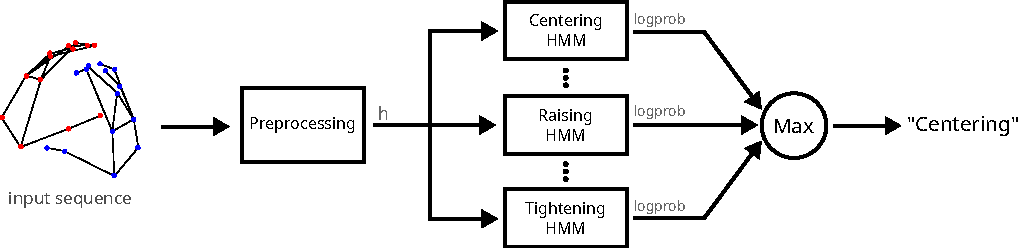
\includegraphics[]{architecture.pdf}
\caption{Architecture of the proposed HMM-based method.}
\label{fig:architecture}
\end{figure*}


\newpage \hbox{} \newpage

%%%%%%%%%%%%%%%%%%%%%%%%%%%%%%%%%%%%%%%%%%%%%%%%%%%%%%%%%%%%%%%%%%%%%%%%%%%%

%% main text
\section{HMM-based classification}

The proposed method utilizes an array of Hidden Markov Models (HMMs) with Gaussian mixture emissions. 

HMMs are known to be particularly well suited for modelling and classifying signals that demonstrate intrinsic temporality, like human speech \citep{rabinerTutorialHiddenMarkov1989} and movement \citep{papadopoulosRealTimeSkeletonTrackingBasedHuman2014}. This makes them a promising choice for the present task of hand action recognition.

\subsection{Architecture}



The basic architecture of the proposed solution is illustrated in \hyperref[fig:architecture]{Fig. 1}. Each input sequence is initially filtered, processed and flattened to a single vector ($h$), which is then fed to $N$ distinct HMMs. Each HMM models one of the observed actions (classes) and, using a scoring function, evaluates the (log) probability of the given input sequence. The most likely match can then be extracted using a simple voting system based on the generated probabilities. \\ 


Each processing step is described in detail in the following paragraphs.

\subsubsection{Preprocessing}

Each of the provided examples is compromised of a sequence of frames, with each frame containing the coordinates of each marker. In order to train the HMMs, each sequence has to be converted to a single vector. Different ways of generating this representation were tested and compared, with the most efficient ultimately being interlacing the position data with estimated velocity data:

\begin{equation}
h_t = [ x_1 \ y_1 \ z_1 \ \Delta x_1 \ \Delta y_1 \ \Delta z_1 \ x_2 \ y_2 \ z_2 \ \Delta x_2 \ \Delta y_2 \ \Delta z_2 \ \cdots \ ]
\end{equation}

\begin{equation}
h = [ h_0 \ h_1 \ h_2 \ \cdots \ ]
\end{equation}


The velocity of each marker is estimated as the difference between the current coordinates of the marker and those of the previous frame. \\

Another useful preprocessing step identified during testing was filtering the data by keeping only markers placed on the subjects fingertips (\textit{THM, IDX, MID, RNG} and \textit{PNK}), wrist (\textit{IWR} and \textit{OWR}) and center of the hand (\textit{IHAND}). This improves training speed without affecting the models performance, as the positions of the other markers seem to provide mostly redundant information. \\

Finally, each sequence can be downsampled by only keeping every $n$ frames. This improves training speed and, in some cases, also improves performance as the delta values become more intensified.

\subsubsection{HMMs}
One fully connected first order HMM is fitted to model the provided training examples of each separate class using the Expectation-Maximization (EM) algorithm \citep{dempsterMaximumLikelihoodIncomplete1977}. The observations for each state are modeled using a Gaussian Mixture Model (GMM) with a full covariance matrix. The number of states of each HMM, as well as the number of states of each GMM are considered free variables. \\

The implementation of HMMs used was provided by the hmmlearn\footnote{\url{https://github.com/hmmlearn/hmmlearn}} python library, while hyperparameter optimization was performed based on leave-one-out cross validation (LOOCV) manually and automcatically using Optuna \citep{akibaOptunaNextgenerationHyperparameter2019}.

\subsubsection{Results}

The best observed result during LOOCV across all 50 examples had an overall accuracy of $90\%$. This translated to $83.\overline{3}\%$ accuracy on the provided test set (10/12).


%%Vancouver style references.
\bibliographystyle{cag-num-names}
\bibliography{refs}



\end{document}

%%
